\documentclass[11pt]{article}
\usepackage[margin=2.2cm]{geometry}
\usepackage{graphicx,booktabs,amsmath,hyperref,xcolor,natbib}
\newcommand{\todo}[1]{\textcolor{red}{[TODO: #1]}}

\title{Less Data, Smaller Model? Data-Constrained Training of Small GPTs under a Fixed Compute Budget}
\author{Timothy Teo Shao Jun (A0272851B) \and Delphino Chew Jing Cheng (A0271802L)\\[4pt]
\small Repository: \url{https://github.com/Teamoreteateo/DSA4212-Small_LLM}}
\date{DSA4212, \todo{date}}

\begin{document}
\maketitle

\paragraph{Declarations (required by the project specification).}
\begin{itemize}
\item \textbf{Compute budget:} a fixed number of training tokens per model, equal to 600\,s of median
  measured training throughput on one NVIDIA Tesla T4 (Section~\ref{sec:budget}); evaluation, tokenizer
  training and pilot runs are excluded. Declared on 27 Oct 2026, before the main experiments.
\item \textbf{Initialisation:} all models are trained from random initialisation; no pretrained weights,
  embeddings or other neural components are used. The tokenizer is trained by us on the training split.
\item \textbf{Evaluation objective:} bits per byte (BPB) on a held-out test set, the second half of the
  official TinyStories validation split, which is never used for tuning.
\end{itemize}

% ===========================================================================
\section{Introduction}
\todo{DRAFT -- rewrite in your own words}
Compute-optimal scaling laws \citep{kaplan2020scaling,hoffmann2022chinchilla} describe how to split a
training budget between model size and training tokens, but they assume that fresh data never runs out.
When unique data is limited, extra compute must be spent either on repeating the same data for more epochs
or on a larger model that passes over it fewer times. \citet{muennighoff2023scaling} studied this trade-off
for models of 10M--9B parameters under FLOP-matched budgets: a few epochs of repetition were almost as good
as new data, the value of repeated tokens decayed after roughly 16 epochs, and under data constraints extra
compute was better spent on epochs than on parameters.

We ask whether the same picture holds for tiny GPTs trained for ten minutes on a single GPU, where the
budget that matters in practice is device time rather than FLOPs:
\begin{quote}\emph{Under a fixed per-run compute budget, how do (i) the optimal model size and (ii) the
usefulness of repeating data change as the number of unique training tokens $U$ shrinks?}\end{quote}
\noindent Two hypotheses were fixed before the main experiments.
\textbf{H1}: the optimal model size decreases as $U$ decreases.
\textbf{H2}: larger models stop benefiting from repetition after fewer epochs.

We train five model sizes (0.4M--25M non-embedding parameters) at four levels of unique data
(1.5M--100M tokens), with three seeds each, plus a dropout follow-up. H2 is supported, with and without
dropout. H1 holds only in part. Without regularisation, the optimum moves non-monotonically
(m4 $\to$ m5 $\to$ m1) and the shift disappears under early stopping, because under a device-time budget
larger models are slower and therefore repeat their data less. With dropout, moderate scarcity (6M tokens)
leaves the optimum unchanged, while extreme scarcity (1.5M tokens) clearly favours the smallest model, which
then achieves the best result of all strategies we tried.

% ===========================================================================
\section{Background}
\todo{DRAFT -- rewrite in your own words after reading the papers}

\paragraph{Compute-optimal scaling.}
\citet{kaplan2020scaling} found that language-model loss follows power laws in parameters, data and compute,
and introduced the convention of counting non-embedding parameters, which we follow.
\citet{hoffmann2022chinchilla} revised the allocation: parameters and training tokens should grow in equal
proportion, which for their models amounted to roughly 20 training tokens per parameter. Both studies assume
each token is seen once.

\paragraph{Repeated data.}
\citet{muennighoff2023scaling} extend the Chinchilla law to repeated data by splitting training tokens into
unique tokens and repetitions, and treating each repetition as worth exponentially less than fresh data
(their \S3). Repeating the whole corpus for up to about four epochs barely changed loss; the fitted
``half-life'' of repeated data corresponds to about 16 epochs, after which returns vanish (\S6). Because
excess parameters lose value faster than repeated data, their fit recommends smaller models trained for more
epochs than Chinchilla would suggest (\S5): the basis of our H1. They also observe that too many epochs or
parameters eventually \emph{increase} loss, which their law does not model: the basis of our H2.
In contrast, \citet{hernandez2022repeated} repeat only a small subset of the data many times and find that this
can hurt performance disproportionately; like \citet{muennighoff2023scaling}, we repeat the entire subset uniformly.

\paragraph{Non-monotonic generalisation.}
\citet{nakkiran2021deep} show that test error can be non-monotonic in model size and in training time
(``double descent''): models just large enough to fit their training data can generalise worse than both
smaller and larger ones. Our 6M results show a similar non-monotonic pattern, although our mechanism differs
because, under a fixed device-time budget, model size and number of epochs change together
(Section~\ref{sec:mechanism}).

\paragraph{Small models and our setting.}
TinyStories \citep{eldan2023tinystories} was built so that models of a few million parameters can learn fluent
English, which makes it suitable for ten-minute runs; our implementation follows nanoGPT
\citep{karpathy2022nanogpt}. Our setting differs from the studies above in three ways: models are about three
orders of magnitude smaller, the data is simple synthetic text rather than web text, and the budget is matched
in device time rather than FLOPs.

% ===========================================================================
\section{Experimental setup}\label{sec:setup}

Our design follows the data-constrained protocol of \citet{muennighoff2023scaling} at a much smaller
scale, with one deliberate difference: the per-run budget is matched in \emph{device time} rather than
in FLOPs (Section~\ref{sec:budget}).

\paragraph{Data.}
We use TinyStories \citep{eldan2023tinystories}, whose simple vocabulary allows models with only a few
million parameters to learn fluent text, making it suitable for ten-minute runs. Training stories are
shuffled once with a fixed seed and tokenised; the first 100M tokens form the training pool.
Each unique-data level $U\in\{100,25,6,1.5\}$M uses the first $U$ tokens of this pool, so smaller
subsets are nested inside larger ones, as in \citet[Fig.~2]{muennighoff2023scaling}: differences
between levels reflect the \emph{amount} of unique data, not its content. The official TinyStories
validation split (21{,}990 stories) is halved: the first half (2.33M tokens) is our validation set, used
only for learning-rate selection and training curves; the second half (2.56M tokens) is the test set,
used only for reported numbers.

\paragraph{Repetition.}
A run cuts its $U$ tokens into non-overlapping 256-token windows and reshuffles them every epoch, so
the entire subset is repeated uniformly and epoch counts are exact. This matches
\citet{muennighoff2023scaling} and avoids the partial up-sampling studied by
\citet{hernandez2022repeated}, where repeating a small fraction of data many times is especially harmful.

\paragraph{Tokenizer.}
A byte-level BPE tokenizer \citep{radford2019gpt2} with a 4096-token vocabulary is trained on 200k
training stories (tokenizer training is excluded from the budget, as permitted). A small vocabulary
keeps the embedding table from dominating tiny models: with GPT-2's 50k vocabulary, m1's embedding
would hold $\approx$6.4M parameters, 16$\times$ its 0.40M non-embedding parameters; with 4096 tokens it
holds 0.52M. The tokenizer averages 3.92 bytes per token on the training data and 3.96 on the validation data.

\paragraph{Models.}
Five pre-LayerNorm GPT models \citep{vaswani2017attention,radford2019gpt2} with tied input/output
embeddings, GELU MLPs of width $4d$, learned positional embeddings, context length 256, and GPT-2
initialisation, following nanoGPT \citep{karpathy2022nanogpt} (Table~\ref{tab:models}). Dropout is 0 except in
the follow-up (Section~\ref{sec:dropout}). We report non-embedding parameter counts, following
\citet{kaplan2020scaling}.

\paragraph{Optimisation.}
AdamW \citep{loshchilov2019adamw} with $\beta=(0.9,0.95)$, weight decay 0.1 on weight matrices only,
gradient clipping at 1.0, batch $64\times256=16{,}384$ tokens, and fp16 mixed precision (the T4 has no
bf16). The learning rate warms up linearly over the first 2\% of the budget and then follows a cosine
decay to 10\% of its peak, the schedule used by \citet{muennighoff2023scaling}. Because the schedule is
defined on the fraction of budget used, every run completes it. Peak learning rates were selected per
model in 17 pilot runs at $U=100$M on the \emph{validation} set (Appendix~\ref{app:lr}): $3\times10^{-3}$
for m1--m4 and $2\times10^{-3}$ for m5, which diverged at $3\times10^{-3}$. A single shared learning rate
was rejected because it would favour some model sizes over others and bias the comparison of optimal size.

\paragraph{Compute budget.}\label{sec:budget}
Each run receives a fixed number of training tokens, equal to 600\,s of that model's median measured
training throughput on an NVIDIA Tesla T4 (Table~\ref{tab:models}). We first timed runs directly, but
throughput for the \emph{same} model varied by up to 24--39\% across cloud hosts, which would have made
results depend on host assignment (Section~\ref{sec:notwork}). Fixing tokens removes this noise while
keeping the budget equal to ten minutes of typical T4 time. The budget was declared before the main
experiments (repository commit of 27 Oct 2026).

Matching device time rather than FLOPs is a deliberate choice: it reflects the cost a practitioner pays
for GPU time. Small models use the GPU less efficiently, so non-embedding training FLOPs ($6ND$) range from
$1.0\times10^{15}$ for m1 to $7.0\times10^{15}$ for m5. Under a FLOP-matched budget, as in
\citet{hoffmann2022chinchilla} and \citet{muennighoff2023scaling}, small models would receive even more tokens.

\begin{table}[h]\centering\small
\caption{Models and per-run budgets. Throughput: median over pilot runs on a T4.
Tokens/param uses non-embedding parameters.}
\label{tab:models}
\begin{tabular}{lrrrrrrrr}\toprule
Model & layers & $d$ & heads & non-emb.\ params & tokens/s & token budget & steps & tokens/param\\\midrule
m1 & 2 & 128 & 4 & 0.40M & 716k & 430M & 26.2k & 1083\\
m2 & 4 & 192 & 4 & 1.78M & 379k & 228M & 13.9k & 128\\
m3 & 6 & 256 & 8 & 4.74M & 234k & 141M & 8.6k & 30\\
m4 & 6 & 384 & 6 & 10.6M & 145k & 87M & 5.3k & 8.2\\
m5 & 8 & 512 & 8 & 25.2M & 76k & 46M & 2.8k & 1.8\\\bottomrule
\end{tabular}\end{table}

\paragraph{Experimental grid.}
We train all 5 models at all 4 values of $U$ with 3 seeds (60 runs). Epochs are not chosen directly:
they equal token budget$/U$ (Table~\ref{tab:epochs}). The $U$ levels were chosen so that the grid spans
the regimes identified by \citet{muennighoff2023scaling}: under 4 epochs (repetition nearly free), around
16 epochs (their estimated half-life of repeated data), and far beyond it, where returns vanish and
overfitting is expected.

\begin{table}[h]\centering\small
\caption{Epochs over the unique data in each cell of the grid (token budget$/U$).}
\label{tab:epochs}
\begin{tabular}{lrrrrr}\toprule
$U$ & m1 & m2 & m3 & m4 & m5\\\midrule
100M & 4.3 & 2.3 & 1.4 & 0.9 & 0.5\\
25M  & 17  & 9.1 & 5.6 & 3.5 & 1.8\\
6M   & 72  & 38  & 24  & 15  & 7.7\\
1.5M & 287 & 152 & 94  & 58  & 31\\\bottomrule
\end{tabular}\end{table}

\paragraph{Evaluation.}
The primary metric is test bits per byte,
$\mathrm{BPB}=\sum_t -\ln p(x_t\mid x_{<t})\,/\,(\ln 2\cdot B)$, where $B$ is the number of UTF-8 bytes of
the predicted tokens, computed on the first 2M test tokens at the final checkpoint. BPB does not depend on
the tokenizer, so results can be compared with other work. Following \citet{muennighoff2023scaling}, we use
no early stopping, so that overfitting remains visible. Training and validation loss are also logged every
30\,s of training time on fixed windows (identical across runs) for the overfitting analysis. BPB measures
next-token prediction only, not the quality of generated stories or performance outside TinyStories. We
report means over 3 seeds with 95\% $t$-intervals. Decision rules for both hypotheses, and a rule for
diverged runs, were fixed before the main grid (\texttt{notes/analysis\_plan.md}). No run met the
divergence rule (seed standard deviation $\le$ 0.015 BPB in every cell).

% ===========================================================================
\section{Results}\label{sec:results}

\subsection{Does the optimal model size shrink with less unique data? (H1)}

\begin{figure}[t]\centering
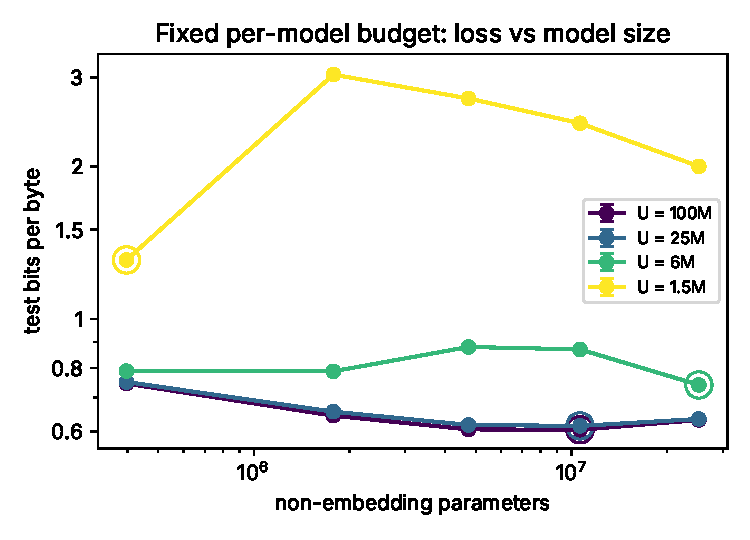
\includegraphics[width=0.49\linewidth]{figures/main_bpb_vs_size.pdf}\hfill
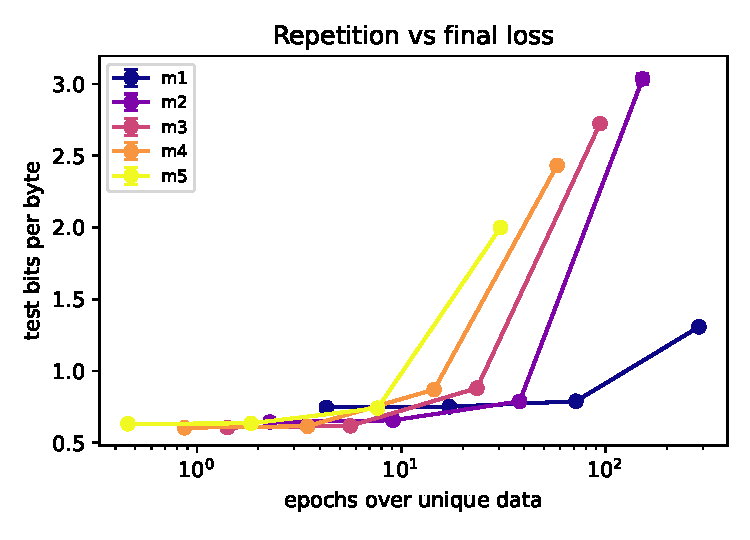
\includegraphics[width=0.49\linewidth]{figures/main_bpb_vs_epochs.pdf}
\caption{Left: test BPB against model size at each $U$ (log axes; circle marks the optimum).
Right: test BPB against epochs over the unique data, one line per model. Error bars: 95\% $t$-intervals over 3 seeds.}
\label{fig:size}\label{fig:epochs}
\end{figure}

\paragraph{Data-rich regime.}
At $U=100$M, m4 (0.604 $\pm$ 0.001 BPB) and m3 (0.605 $\pm$ 0.003) are tied for the lowest test BPB
(Fig.~\ref{fig:size}, left; Table~\ref{tab:main}). They see 8 and 30 tokens per non-embedding parameter,
bracketing the $\approx$20 tokens per parameter that \citet{hoffmann2022chinchilla} find
compute-optimal.\footnote{The bracket also holds if embedding parameters are counted: m3 then has 5.9M
parameters (24 tokens/param) and m4 12.3M (7.1 tokens/param).}
Both the smallest model (m1, 1083 tokens/param) and the largest (m5, 1.8 tokens/param) are clearly worse,
so the optimum lies inside our model range. The ranking at $U=25$M is the same (m4 0.615, m3 0.618).

\paragraph{Repetition up to a few epochs is nearly free.}
Going from $U=100$M to 25M means every model repeats its data about four times more often. Test BPB rises by
only 0.5\% for m5 (1.8 epochs), 0.7\% for m1 (17 epochs) and 1.8--2.0\% for m2--m4 (3.5--9 epochs).
These differences exceed the confidence intervals but are small in practice, consistent with the finding of
\citet{muennighoff2023scaling} that up to about four epochs of repeated data is worth almost as much as fresh data.

\paragraph{Scarce data: a non-monotonic path.}
At $U=6$M the optimum moves \emph{up} to the largest model, m5 (0.741 $\pm$ 0.005), ahead of m1 and m2
($\approx$0.79), while the mid-sized m3 and m4 are worst (0.88 and 0.87). At $U=1.5$M it collapses to the
smallest model, m1 (1.307 $\pm$ 0.015), with m2 the worst at 3.04 BPB, close to the $\approx$3.06 BPB of a
uniform guess over the vocabulary ($\log_2 4096 / 3.92$). By our pre-registered rule H1 is supported: the
optimum at 1.5M (m1) is smaller than the optimum at 100M (m4), and at 1.5M their intervals are far apart
(1.307 $\pm$ 0.015 vs.\ 2.433 $\pm$ 0.019). The 6M row, however, shows that the optimum does not shrink
smoothly, and Section~\ref{sec:mechanism} shows that the result depends on training to the end of the budget.

\begin{table}[h]\centering\small
\caption{Test BPB (mean over 3 seeds; 95\% interval half-width $\le$ 0.036 in every cell). Bold: optimum per row.}
\label{tab:main}
\begin{tabular}{lrrrrr}\toprule
$U$ & m1 & m2 & m3 & m4 & m5\\\midrule
100M & 0.745 & 0.644 & 0.605 & \textbf{0.604} & 0.632\\
25M  & 0.751 & 0.656 & 0.618 & \textbf{0.615} & 0.635\\
6M   & 0.789 & 0.788 & 0.880 & 0.870 & \textbf{0.741}\\
1.5M & \textbf{1.307} & 3.036 & 2.723 & 2.433 & 2.000\\\bottomrule
\end{tabular}\end{table}

\subsection{When does repetition stop helping? (H2)}

We measure overfitting onset as the number of epochs at which validation loss reaches its minimum, counted
only when it later rises by more than 0.005 nats. At $U=6$M, onset falls steadily with model size: 23.2, 12.4,
8.2 and 5.7 epochs for m2--m5, while m1 never overfits in 72 epochs. At $U=1.5$M it is 28.5, 15.8, 9.1, 8.8 and
7.3 epochs for m1--m5, after which validation loss rises by 0.9 (m1) to 5.7 (m2) nats. H2 is therefore
supported: larger models stop benefiting from repetition sooner. Because losses are logged every 30\,s of
training, onset is resolved only to about 1/20 of a run's epochs. This is fine at 6M (0.4--1.9 epochs), but at
1.5M m3, m4 and m5 cannot be told apart. The secondary measure, the final gap between validation and training
loss, is not monotonic in size at 1.5M (m2 has the largest gap) because it depends on how many epochs a model
trains \emph{past} its onset, not only on when overfitting starts.

\subsection{Mechanism: size and repetition are coupled}\label{sec:mechanism}

Under a fixed device-time budget a larger model is slower, so it sees fewer epochs of the same data. Combining
this with H2 explains the H1 pattern. At 6M, m3 and m4 run 24 and 15 epochs, well past their onsets (12 and 8),
and their validation loss rises by 0.40 nats; m5 runs only 7.7 epochs, just past its onset (5.7), and loses 0.08.
The largest model wins because its slowness protects it from over-repetition, while m1 and m2 have too little
capacity to memorise much. At 1.5M every model passes its onset by a wide margin, and only m1's tiny capacity
limits the damage.

\paragraph{Sensitivity check: early stopping.}
As pre-registered, we re-rank models by their best validation loss (an early-stopped checkpoint) instead of the
final one (\texttt{results/tables/early\_stop\_check.csv}). The ranking is unchanged at 100M and 25M, but at the
small $U$ levels it reverses: at 6M the order becomes m5, m4, m3, m2, m1, and at 1.5M m4 and m5 are best and m1
is \emph{last}. Without regularisation, the shrinking optimum in H1 therefore depends on training every model to
the end of its budget: early stopping alone favours larger models at small $U$. Section~\ref{sec:dropout} shows
that this changes once overfitting is controlled by dropout. This check ranks seed-mean validation losses without
intervals, and selecting the best checkpoint on the validation set is slightly optimistic, so it supports a
qualitative conclusion only.

\subsection{Follow-up: does regularisation change the optimum?}\label{sec:dropout}

If over-repetition drives the H1 pattern, regularisation should change it. We reran all five models at
$U\in\{6,1.5\}$M with dropout 0.1 \citep{srivastava2014dropout}, keeping budgets and learning rates fixed
(30 runs; Table~\ref{tab:dropout}). The pre-registered follow-up covered m3 and m5; m4 and then m1, m2 were
added to complete the comparison (commit history).

\paragraph{Moderate scarcity (6M): the reversal disappears.}
Dropout improves m2--m5 by 0.06--0.19 BPB and removes overfitting almost entirely (validation loss rises by at
most 0.006 nats). The optimum returns to m4 (0.681 $\pm$ 0.002), clearly ahead of m5 (0.685 $\pm$ 0.001), the
same model that is optimal at 100M and 25M. Once overfitting is controlled, moderate data scarcity does not
move the optimum. Dropout also outperforms early stopping here: the best early-stopped model without dropout
(m5) reaches $\approx$0.72 BPB, against 0.681 for m4 with dropout. Dropout slightly \emph{hurts} m1
(0.789 $\to$ 0.802): the smallest model was not overfitting, so regularisation only removes capacity it needs.

\paragraph{Extreme scarcity (1.5M): the smallest model wins, and wins by more.}
Dropout lowers test BPB for every model, by 33\% (m1) to 70\% (m2), and the ranking becomes almost monotonic
in size: m1 (0.874 $\pm$ 0.004) $<$ m2 (0.921) $<$ m3 (1.151) $<$ m5 (1.290) $<$ m4 (1.355). m1 is best both at
the final checkpoint and under early stopping, unlike without dropout, where early stopping put m1 last.
m1 with dropout is also clearly better than the best early-stopped model without dropout (m4, $\approx$0.94 BPB,
converted from validation loss using 3.96 bytes per validation token; validation BPB runs about 0.01 above test
BPB on the same runs, so the gap of $\approx$0.06--0.07 BPB is not an artefact of the split). With
regularisation, extreme data scarcity therefore does favour the smallest model, which supports H1 more strongly
than the unregularised grid.

\paragraph{H2 under dropout.}
Dropout delays overfitting but does not prevent it at 1.5M: onset falls with size (37.9, 17.2, 13.9 and 10.1
epochs for m2--m5; m1 never overfits) and validation loss still rises by 0.1--1.3 nats afterwards. H2 thus holds
with and without regularisation.

\begin{table}[h]\centering\small
\caption{Test BPB without and with dropout 0.1 (mean over 3 seeds; 95\% half-width $\le$ 0.036).
Bold: best per column.}
\label{tab:dropout}
\begin{tabular}{lrrrr}\toprule
 & \multicolumn{2}{c}{$U=6$M} & \multicolumn{2}{c}{$U=1.5$M}\\
Model & none & 0.1 & none & 0.1\\\midrule
m1 & 0.789 & 0.802 & \textbf{1.307} & \textbf{0.874}\\
m2 & 0.788 & 0.713 & 3.036 & 0.921\\
m3 & 0.880 & 0.687 & 2.723 & 1.151\\
m4 & 0.870 & \textbf{0.681} & 2.433 & 1.355\\
m5 & \textbf{0.741} & 0.685 & 2.000 & 1.290\\\bottomrule
\end{tabular}\end{table}

% ===========================================================================
\section{What did not work and unexpected results}\label{sec:notwork}
\todo{DRAFT -- rewrite in your own words; all items are from notes/experiment\_log.md}
\begin{itemize}
\item \textbf{Wall-clock budgets were unreliable on shared cloud GPUs.} In the learning-rate pilots, throughput
  for the same model varied across Modal T4 hosts by 24\% (m5: 67k--83k tokens/s) and 39\% (m4: 109k--152k).
  One m4 run at learning rate $2\times10^{-3}$ landed on a slow host, completed about 30\% fewer steps, and
  appeared worse than both neighbouring learning rates. Since this noise rivalled the effects we wanted to
  measure (m3 vs.\ m4 at 100M differ by 0.001 BPB), we replaced live timing with a fixed per-model token budget.
\item \textbf{Instability of the largest model.} m5 diverged at learning rate $3\times10^{-3}$ within the first
  minute and never recovered (final validation loss 3.45 vs.\ 1.76 at $2\times10^{-3}$), likely due to fp16
  training at a high learning rate, so m5 uses a lower peak learning rate than m1--m4.
\item \textbf{Learning-rate optima at the grid edge.} The first pilot found the best learning rate at the edge
  of the grid for m1 and m3, so a second pilot was needed to confirm interior optima.
\item \textbf{The 6M reversal contradicted H1.} We expected the optimum to shrink smoothly with $U$; instead it
  moved to the largest model at 6M. Investigating this led to the coupling mechanism and the dropout follow-up,
  which removed the reversal.
\item \textbf{Catastrophic memorisation.} m2 at 1.5M reached 3.04 test BPB, about the level of a uniform guess,
  showing that repeated data can make a model extremely overconfident rather than merely less accurate.
\item \textbf{Dropout is not free.} At 6M, dropout made m1 slightly worse (0.789 $\to$ 0.802 BPB), because the
  smallest model was capacity-limited rather than overfitting. A single dropout rate is not optimal for every
  model size.
\item \textbf{Re-running is not bit-exact.} The dropout runs for m3--m5 were executed twice; results differed
  slightly (e.g.\ m5 at 1.5M: 1.288 vs.\ 1.290 BPB) but always within the 95\% intervals, consistent with GPU
  non-determinism. We report the latest runs.
\end{itemize}

% ===========================================================================
\section{Limitations}
\begin{itemize}
\item \textbf{One dataset.} TinyStories is simple and repetitive; overfitting onsets may differ on web text.
\item \textbf{Scale.} Our models are about three orders of magnitude smaller than those of
  \citet{muennighoff2023scaling}, and budgets are minutes rather than GPU-months.
\item \textbf{Device-time budget.} Results depend on the hardware's relative throughput across model sizes;
  a FLOP-matched budget would give small models more tokens and could change the optimum.
\item \textbf{Hyperparameters.} Learning rates were tuned at $U=100$M without dropout and reused at all $U$ and in
  the dropout runs; only one dropout rate (0.1) was tried, and dropout was not run at 100M or 25M, so we cannot
  say whether it would change the data-rich optimum. m2's budget is based on only two throughput measurements.
\item \textbf{Measurement.} Overfitting onset is resolved to about 1/20 of a run; the early-stopping check uses
  validation loss without intervals; 3 seeds per cell.
\item \textbf{Final checkpoint.} Our main metric uses the final checkpoint; Section~\ref{sec:mechanism} shows this
  choice drives the unregularised H1 result at small $U$.
\end{itemize}

% ===========================================================================
\section{Use of AI tools}
\todo{DRAFT -- edit so every statement is true for your group}
We used Claude (Anthropic), in chat and through Claude Code, to draft the training, analysis and cloud-runner
code; to suggest checks (a token-budget smoke test, the early-stopping sensitivity analysis and the
bytes-per-token conversion); and to draft the Setup, Results and Background sections and our reading notes
from our configuration and result files. We reviewed and tested all code, ran all experiments ourselves,
verified every reported number against the result tables in the repository, checked cited claims against the
original papers, and rewrote \todo{which sections} in our own words. The research question, the decision to
replace wall-clock timing with a token budget, the per-model learning rates, and the extension of the dropout
follow-up to all five models were \todo{confirm: our decisions / made with AI suggestions that we evaluated}.

% ===========================================================================
\section{Conclusion}
\todo{DRAFT -- rewrite in your own words}
Larger models stop benefiting from repeated data after fewer epochs, with and without regularisation (H2).
Whether scarce data calls for a smaller model (H1) depends on how overfitting is handled. Without
regularisation, the optimum moves non-monotonically because, under a device-time budget, larger models are
slower and therefore repeat their data less, and early stopping alone reverses the trend. With dropout,
moderate scarcity leaves the optimum unchanged, while extreme scarcity clearly favours the smallest model,
which achieves the best result we observed at that data level. An open question is whether these conclusions
survive a FLOP-matched budget, under which small models would see even more tokens, and data that is harder
to memorise than TinyStories.

\bibliographystyle{plainnat}
\bibliography{refs}

% ===========================================================================
\appendix
\section{Learning-rate pilots}\label{app:lr}
Final validation loss (nats/token) at $U=100$M, one seed per cell, from \texttt{results/tables/lr\_sweep.csv}.
These runs are excluded from the compute budget, as permitted.

\begin{table}[h]\centering\small
\begin{tabular}{lrrrrr}\toprule
Model & $3\times10^{-4}$ & $10^{-3}$ & $2\times10^{-3}$ & $3\times10^{-3}$ & $6\times10^{-3}$\\\midrule
m1 & 2.243 & 2.089 & -- & \textbf{2.056} & 2.065\\
m2 & -- & -- & -- & \textbf{1.783} & 1.795\\
m3 & 1.863 & 1.718 & -- & \textbf{1.685} & 1.698\\
m4 & -- & 1.700 & 1.733$^\dagger$ & \textbf{1.674} & --\\
m5 & 1.861 & 1.792 & \textbf{1.763} & 3.454$^\ddagger$ & --\\\bottomrule
\end{tabular}

\smallskip
{\footnotesize $^\dagger$ slow host, $\approx$30\% fewer steps (run made before the switch to token budgets).
$^\ddagger$ diverged.}
\end{table}

\section{Additional figures}
\begin{figure}[h]\centering
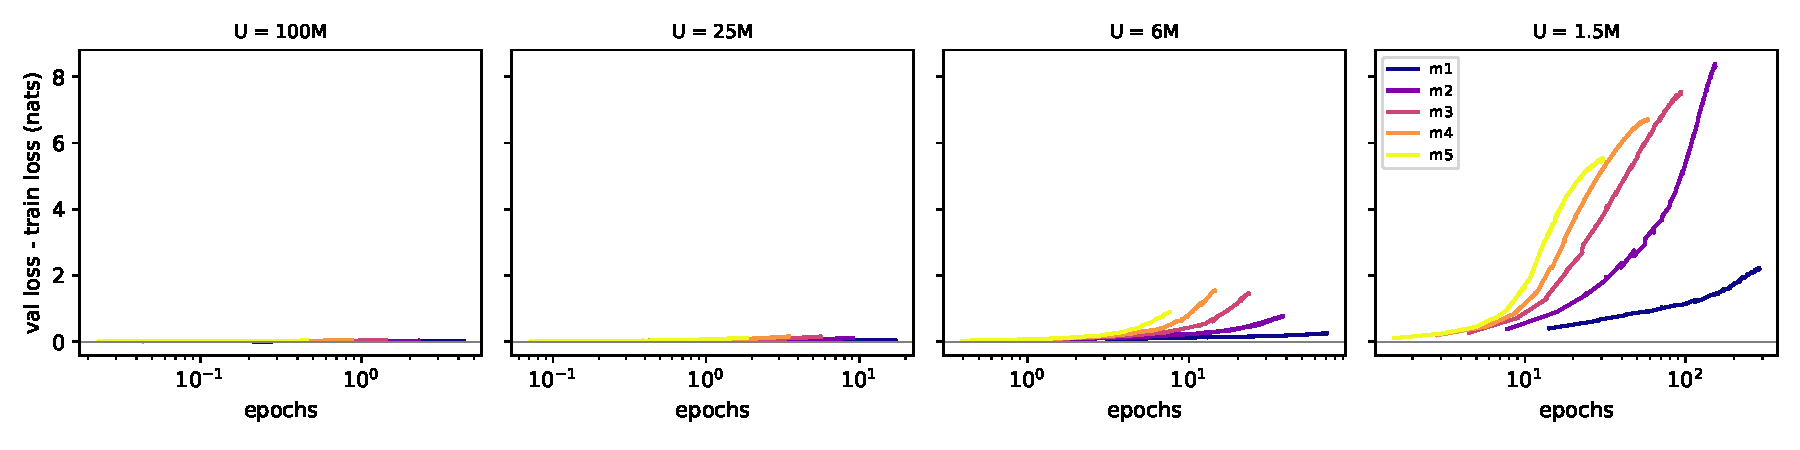
\includegraphics[width=0.95\linewidth]{figures/main_gap_vs_epochs.pdf}
\caption{Validation minus training loss during training, by $U$ (no dropout).}
\end{figure}
\begin{figure}[h]\centering
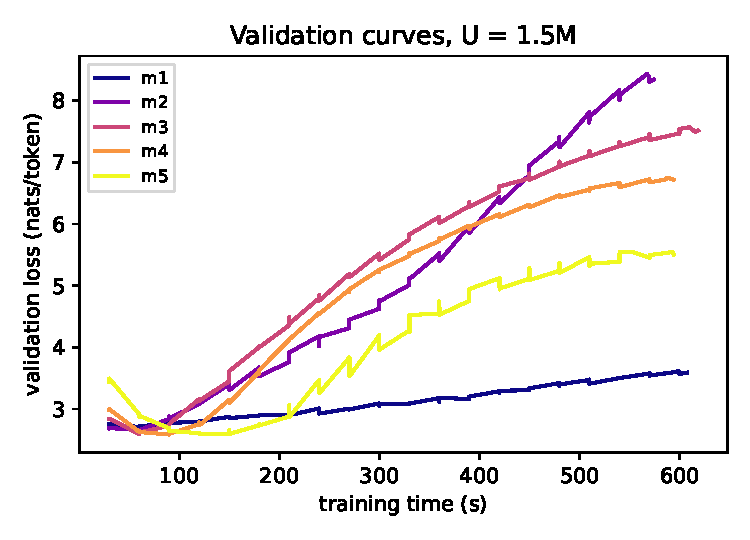
\includegraphics[width=0.6\linewidth]{figures/main_val_curves_smallU.pdf}
\caption{Validation curves at $U=1.5$M (mean $\pm$ s.d.\ over seeds; no dropout).}
\end{figure}

\end{document}